
\section{shallow ice sheets}

\begin{frame}{slow, non-Newtonian, shallow, and sliding}

\begin{itemize}
\item ice sheets have four outstanding properties \emph{as fluids}:
  \begin{enumerate}
  \item slow
  \item non-Newtonian
  \item shallow (usually)
  \item contact slip (sometimes)
  \end{enumerate}
\end{itemize}
\end{frame}


\begin{frame}{regarding ``shallow''}

\begin{itemize}
\item in \alert{red} is a Greenland cross section
  \begin{itemize}
  \item[$\circ$] at $71^\circ$ N: \qquad width = 760 km, thickness = 3200 m
  \end{itemize}
\item green and blue: standard vertically-exaggerated cross section
\end{itemize}

\begin{center}
  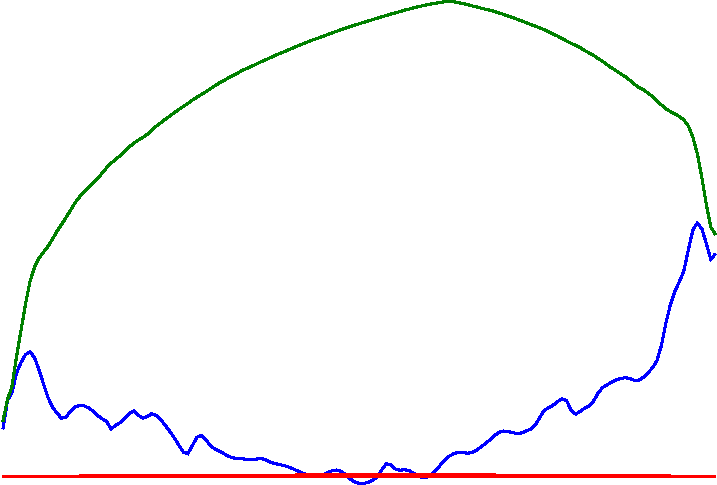
\includegraphics[width=0.85\textwidth]{green-transect}
\end{center}
\end{frame}


\begin{frame}{flow model I: shallow ice approximation (SIA)}

a model which applies to
\begin{itemize}
\item small depth-to-width ratio (``shallow'') grounded ice sheets
\item for \emph{not}\, too rough/steep bed topography
\item when flow is \emph{not}\, dominated by sliding at the base
\end{itemize}

\begin{center}
  \includegraphics[width=0.7\textwidth]{polaris}

\tiny ``Polaris Glacier,'' northwest Greenland, photo 122, Post \& LaChapelle (2000)
\end{center}

\end{frame}


\begin{frame}{SIA model equations}

\begin{itemize}
\item simple slogan: \emph{the SIA uses the formulas from slab-on-a-slope}
  \begin{itemize}
  \item[$\circ$] better explanation: expand the Stokes equations in aspect ratio
  \end{itemize}

\item shear stress approximation:
	$$(\tau_{13},\tau_{23}) = - \rho g (h-z) \nabla h$$
\item then horizontal velocity $\mathbf{u} = (u,v)$ satisfies this approximation:
\begin{align*}
\mathbf{u}_z &= 2 A |(\tau_{13},\tau_{23})|^{n-1} (\tau_{13},\tau_{23}) \\
     &= - 2 A (\rho g)^n (h-z)^n |\nabla h|^{n-1} \nabla h
\end{align*}
\item by integrating vertically (non-sliding case):
    $$\mathbf{u} = - \frac{2 A (\rho g)^n}{n+1} \left[H^{n+1} - (h-z)^{n+1}\right] |\nabla h|^{n-1} \nabla h$$
\item add mass continuity: \quad $H_t = M - \left(\overline{\mathbf{u}} H\right)_x$
\end{itemize}
\end{frame}


\begin{frame}{SIA thickness equation}

\begin{itemize}
\item thus the non-sliding, isothermal SIA for thickness evolution:
\begin{empheq}[box=\fbox]{equation}
H_t = M + \Div \left(\Gamma H^{n+2} |\grad h|^{n-1} \grad h \right) \label{sia}
\end{empheq}

\vspace{-2mm}
  \begin{itemize}
  \item[$\circ$] $H$ is ice thickness, $h$ is ice surface elevation
  \item[$\circ$] \dots also $b$ is bed elevation and $h=H+b$
  \item[$\circ$] $M$ combines surface and basal mass (im)balance
  \item[$\circ$] $\Gamma = 2 A (\rho g)^n / (n+2)$ is a constant
  \end{itemize}
\item \begin{minipage}[t]{0.53\textwidth}
numerically solve (1) and you have a usable model for \dots \emph{the Barnes ice cap}, a boring ice sheet (Mahaffy, 1976) \hfill $\longrightarrow$
\end{minipage}
\end{itemize}
\bigskip \bigskip

\noindent good questions:
\begin{itemize}
\item[] how to solve (1) numerically?
\item[] how to \emph{think} about it?
\end{itemize}

\vspace{-43mm}
\hfill \includegraphics[width=0.34\textwidth]{mahaffy-profiles}
\end{frame}


\begin{frame}{heat equation}
\label{slide:heatcompare}

\small
\begin{columns}
\begin{column}{0.7\textwidth}
\begin{itemize}
\item to understand SIA, see heat equation
\item recall Newton's law of cooling
	$$\frac{dT}{dt} = -K (T-T_{\text{ambient}})$$
where $T$ is object temperature and $K$ relates to material and geometry of object
\item Newton's law for segments of a rod has $T_{\text{ambient}}$ as neighbor average:
\begin{align*}
\frac{dT_j}{dt} &= -K \left(T_j - \frac{1}{2} (T_{j-1} + T_{j+1}) \right) \\
	&= \frac{K}{2} \left(T_{j-1} - 2 T_j + T_{j+1}\right) 
\end{align*}
\item the limit as segments shrink is the \emph{heat equation}:
	$$T_t = D T_{xx}$$
\end{itemize}
\end{column}

\begin{column}{0.3\textwidth}
\hfill \includegraphics[width=0.75\textwidth]{coffee}

\vspace{0.4in}
\includegraphics[width=1.1\textwidth]{heatconduction}
\end{column}
\end{columns}
\end{frame}

\begin{frame}{major analogy: SIA versus 2D heat equation}

\begin{itemize}
\item general 2D heat eqn: \quad $T_t = F + \Div (D\, \grad T)$
\item side-by-side comparison:

\medskip
\begin{tabular}{cc}
\scriptsize SIA for ice thickness \, $H(t,x,y)$ & \scriptsize heat eqn for temperature $T(t,x,y)$ \normalsize \medskip \\
	\hspace{-6mm} $H_t = M + \Div \left({\color{red}\Gamma H^{n+2} |\grad h|^{n-1}}\, \grad h \right)$  &  $T_t = F + \Div (D\, \grad T)$
\end{tabular} 

\medskip
\item identify the diffusivity in the SIA:
	$$D = {\color{red}\Gamma H^{n+2} |\grad h|^{n-1}}$$
\item non-sliding shallow ice flow \emph{diffuses} the ice sheet geometry
\item concerns about this analogy:
  \begin{itemize}
  \item[$\circ$]  $D$ depends on solution $H(t,x,y)$
  \item[$\circ$]  $D\to 0$ at margin, where $H\to 0$
  \item[$\circ$]  $D\to 0$ at divides/domes, where $|\grad h|\to 0$
  \end{itemize}
\end{itemize}
\end{frame}


\begin{frame}{numerics for heat equation: basic finite differences}

\begin{itemize}
\item numerical schemes for heat equation are good start for SIA
\item only \emph{finite difference} (FD) schemes in these slides

\bigskip
\item first, for differentiable $f(x)$ \emph{Taylor's theorem} says
	$$f(x+h) = f(x) + f'(x) h + \frac{1}{2} f''(x) h^2 + \frac{1}{3!} f'''(x) h^3 + \dots$$
\normalsize
\item you can replace ``$h$'' by multiples of $\Delta x$, e.g.:
\small
\begin{align*}
f(x-\Delta x) &= f(x) - f'(x) \Delta x + \frac{1}{2} f''(x) \Delta x^2 - \frac{1}{3!} f'''(x) \Delta x^3 + \dots \\
f(x+2\Delta x) &= f(x) + 2 f'(x) \Delta x + 2 f''(x) \Delta x^2 + \frac{4}{3} f'''(x) \Delta x^3 + \dots
\end{align*}
\normalsize
\item \emph{main idea for FD schemes}:  combine expressions like these to approximate derivatives from the values of functions on a grid
\end{itemize}
\end{frame}


\begin{frame}{partial derivatives}

\begin{itemize}
\item we want FD approximations of partial derivatives
\item for example, with any function $u=u(t,x)$:
\small
\begin{align*}
u_t(t,x) &= \frac{u(t+\Delta t,x) - u(t,x)}{\Delta t} + O(\Delta t), \\
u_t(t,x) &= \frac{u(t+\Delta t,x) - u(t-\Delta t,x)}{2\Delta t} + O(\Delta t^2), \\
u_x(t,x) &= \frac{u(t,x+\Delta x) - u(t,x-\Delta x)}{2\Delta x} + O(\Delta x^2), \\
u_{xx}(t,x) &= \frac{u(t,x+\Delta x) - 2 u(t,x) + u(t,x-\Delta x)}{\Delta x^2} + O(\Delta x^2)
\end{align*}
\normalsize
\item sometimes we want a derivative in-between grid points:
\small
	$$u_x(t,x+\tfrac{\Delta x}{2}) = \frac{u(t,x+\Delta x) - u(t,x)}{\Delta x} + O(\Delta x^2)$$
\normalsize
\item \emph{note}: ``$+O(h^2)$'' is better than ``$+O(h)$'' if $h$ is a small number
\end{itemize}
\end{frame}


\begin{frame}{explicit scheme for heat equation}
\label{slide:explicit}

\begin{itemize}
\item consider 1D heat equation $T_t = D T_{xx}$
\item thus this is approximately true:
\small
	$$\frac{T(t+\Delta t,x) - T(t,x)}{\Delta t} \approx D\,\frac{T(t,x+\Delta x) - 2 T(t,x) + T(t,x-\Delta x)}{\Delta x^2}$$
\normalsize
\item the difference between $T_t = D T_{xx}$ and the scheme is $O(\Delta t,\Delta x^2)$
\item notation:
    \begin{itemize}
    \item[$\circ$] $(t_n,x_j)$ is a point in the time-space grid
    \item[$\circ$] $T_j^n \approx T(t_n,x_j)$  \only<2>{\hfill \alert{$\longleftarrow$ can you distinguish these?}}
    \end{itemize} 
\item let $\mu = D \Delta t / (\Delta x)^2$, so ``explicit'' scheme is
\small
	$$T_j^{n+1} = \mu T_{j+1}^n + (1 - 2 \mu) T_j^n + \mu T_{j-1}^n \phantom{sdfkj sdkfj asdlfj asldkfj asdflkj}$$
\normalsize
\item ``stencil'' at right \large $\to$ \normalsize
\end{itemize}

\vspace{-12mm}
\hfill \includegraphics[width=0.28\textwidth]{expstencil}
\end{frame}


\begin{frame}{explicit scheme in 2D}

\begin{itemize}
\item recall heat equation two spatial variables (2D):
    $$T_t = D(T_{xx} + T_{yy})$$
\item again: $T_{jk}^n \approx T(t_n,x_j,y_k)$
\item the 2D explicit scheme is
\small
	$$\frac{T_{jk}^{n+1} - T_{jk}^n}{\Delta t} = D\,\left(\frac{T_{j+1,k}^n - 2 T_{jk}^n + T_{j-1,k}^n}{\Delta x^2} + \frac{T_{j,k+1}^n - 2 T_{jk}^n + T_{j,k-1}^n}{\Delta y^2}\right)$$
\normalsize
\item which becomes a computable iteration:
\small
	$$T_{jk}^{n+1} = T_{jk}^n + \mu_x (T_{j+1,k}^n - 2 T_{jk}^n + T_{j-1,k}^n) + \mu_y (T_{j,k+1}^n - 2 T_{jk}^n + T_{j,k-1}^n)$$
\normalsize
where $\mu_x=D\Delta t/\Delta x^2$ and $\mu_y = D\Delta t/\Delta y^2$
\end{itemize}

\begin{center}
\includegraphics[width=0.25\textwidth]{exp2dstencil}
\end{center}
\end{frame}


\begin{frame}{implementation}
\label{slide:heatmatlab}

\minput{heat}

\small
\begin{itemize}
\item solves $T_t = D(T_{xx} + T_{yy})$ on square $-1 < x < 1$, $-1 < y < 1$
\item example uses initial condition $T_0(x,y) = e^{-30 r^2}$
\item code uses ``colon notation'' to remove loops (over space)
\end{itemize}
\end{frame}


\begin{frame}{the look of success}

\begin{itemize}
\item \texttt{>>  heat(1.0,30,30,0.001,20)}

\medskip
solves $T_t = D(T_{xx} + T_{yy})$ for $T(t,x,y)$ with $D=1$, $30\times 30$ grid, $\Delta t = 0.001$, and $N=20$ time steps
\end{itemize}

\bigskip
\begin{columns}
\begin{column}{0.5\textwidth}
initial condition $T(0,x,y)$

\bigskip
\begin{center}
\includegraphics[width=1.0\textwidth]{initialheat}
\end{center}
\end{column}
\begin{column}{0.5\textwidth}
\mbox{approximate solution $T(0.02,x,y)$}

\bigskip
\begin{center}
\includegraphics[width=1.0\textwidth]{finalheat}
\end{center}
\end{column}
\end{columns}
\end{frame}


\begin{frame}{the look of instability}

results from solving $T_t = D(T_{xx} + T_{yy})$ on the \emph{same} space grid and at the \emph{same} time, but with slightly-different time steps:

\bigskip
\begin{columns}
\begin{column}{0.5\textwidth}
\begin{center}
\includegraphics[width=1.0\textwidth]{stability}

\uncover<2->{$$\frac{D\Delta t}{\Delta x^2}= 0.2$$}
\end{center}
\end{column}
\begin{column}{0.5\textwidth}
\begin{center}
\includegraphics[width=1.0\textwidth]{instability}

\uncover<2->{$$\frac{D\Delta t}{\Delta x^2}= 0.4$$}
\end{center}
\end{column}
\end{columns}
\end{frame}


\begin{frame}{avoid the instability}
\label{slide:maxprinc}

\begin{itemize}
\item recall 1D explicit scheme had the form 
	$$T_j^{n+1} = \mu T_{j+1}^n + (1 - 2 \mu) T_j^n + \mu T_{j-1}^n$$
\item thus the new value $u_j^{n+1}$ is an \emph{average} of the old values, \emph{if the middle coefficient is positive}:
	$$1 - 2 \mu \ge 0 \quad \iff \quad  \frac{D\Delta t}{\Delta x^2} \le \frac{1}{2} \quad \iff \quad \Delta t \le \frac{\Delta x^2}{2 D}$$
    \begin{itemize}
    \item[$\circ$] this condition is a sufficient \emph{stability criterion}
    \end{itemize}
\item averaging is stable because averaged wiggles are smaller than wiggles
\item instability is because \emph{the time step is too big}
\end{itemize}
\end{frame}


\begin{frame}{\textsl{adaptive} implementation: guaranteed stability}

\minput{heatadapt}

\begin{itemize}
\item same as \texttt{heat.m} except:

\begin{center}
\emph{choose time step from stability criterion}
\end{center}
\end{itemize}\end{frame}


\begin{frame}{alternative instability fix: implicitness}

\begin{itemize}
\item \alert{implicit} methods can be designed to be stable for \emph{any} positive time step $\Delta t$
\item example is \emph{Crank-Nicolson} scheme $\longrightarrow$

\vspace{-7mm}
\hfill \includegraphics[width=0.35\textwidth]{cnstencil}

\vspace{-5mm}
\item has smaller error too: $O(\Delta t^2,\Delta x^2)$
\item \emph{but} you must solve linear (or nonlinear) systems of equations to take each time step

\bigskip

\small
\item Donald Knuth has advice for ice sheet modelers:

\begin{center}
\emph{\dots forget about small efficiencies \dots}

\emph{premature optimization is the root of all evil}
\end{center}

    \begin{itemize}
    \item[$\circ$] I've followed this advice: Bueler et al.~(2005) and PISM use adaptive explicit, Bueler (2016) used implicit    
    \end{itemize}
\end{itemize}
\end{frame}


\begin{frame}{variable diffusivity and staggered grids}

\begin{itemize}
  \item since SIA has diffusivity which varies in space \dots
  \item consider the generalized diffusion/heat equation:
     $$T_t = F + \Div \big(D(x,y) \grad (T+b)\big)$$
  \item an explicit method is conditionally stable, with same condition, if we evaluate diffusivity $D(x,y)$ at \alert{staggered} grid points:
  \small
\begin{align*}
\Div \left(D(x,y) \grad X\right) &\approx \frac{D_{j+1/2,k}(X_{j+1,k} - X_{j,k}) - D_{j-1/2,k}(X_{j,k} - X_{j-1,k})}{\Delta x^2} \\
	&\qquad + \frac{D_{j,k+1/2}(X_{j,k+1} - X_{j,k}) - D_{j,k-1/2}(X_{j,k} - X_{j,k-1})}{\Delta y^2}
\end{align*}
\normalsize
where $X=T+b$
\item in stencil at right $\longrightarrow$
    \begin{itemize}
    \item[] diamonds: $T,b$
    \item[] triangles: $D$
    \end{itemize}

\vspace{-15mm}
\hfill \includegraphics[width=0.3\textwidth]{diffstencil}
\end{itemize}
\end{frame}


\begin{frame}
  \frametitle{general diffusion equation code}

\minputtiny{diffstag}

\small
\begin{itemize}
\item solves abstract diffusion equation $T_t = \Div \left(D(x,y)\, \grad (T+b)\right)$
\item user supplies diffusivity on staggered grid
\end{itemize}
\end{frame}


\begin{frame}{interruption: verification}
\begin{itemize}
\item how do you make sure your \emph{implemented} numerical ice flow code is correct?
  \begin{itemize}
  \item[$\circ$] \emph{technique} 1 = \alert{infallibility}: don't make any mistakes
  \item[$\circ$] \emph{technique} 2 = \alert{intercomparison}: compare your model with others, and hope that the outliers are the ones with errors
  \item[$\circ$] \emph{technique} 3 = \alert{verification}: build-in a comparison to an exact solution, and actually measure the numerical error
  \end{itemize}

\medskip
\item where to get exact solutions for ice flow models?
  \begin{itemize}
  \item[$\circ$] textbooks: Greve and Blatter (2009), van der Veen (2013)
  \item[$\circ$] manufactured solns to thermo-coupled SIA (Bueler et al 2007)
  \item[$\circ$] flowline and cross-flow SSA solns (Bodvardsson, 1955; van der Veen, 1985; Schoof, 2006; Bueler 2014)
  \item[$\circ$] flowline Blatter solns (Glowinski and Rappaz 2003)
  \item[$\circ$] constant viscosity flowline Stokes solns (Ladyzhenskaya 1963, Balise and Raymond 1985)
  \item[$\circ$] manufactured solns to Stokes equations (Sargent and Fastook 2010; Jouvet and Rappaz 2011; Leng et al 2013)
  \end{itemize}
\end{itemize}
\end{frame}


\begin{frame}{the Green's function of the heat equation}

\begin{itemize}
\item recall heat equation in 1D with constant diffusivity $D>0$ is:
	$$T_t = D T_{xx}$$
\item many exact solutions are known!
\item Green's function solution shown below
  \begin{itemize}
  \item[$\circ$] a.k.a.~``fundamental solution'' or ``heat kernel''
  \end{itemize}
\item starts at time $t=0$ with a ``delta function'' $T(0,x)=\delta_0(x)$
\item then it spreads out over time
\end{itemize}

\begin{center}
\includegraphics[width=0.5\textwidth]{heatscaling}

\emph{increasing time} \Large $\to$
\end{center}
\end{frame}


\begin{frame}{the Green's function of the heat equation \quad 2}

\begin{itemize}
\item the Green's function can be found by a method which generalizes to the SIA: the solution is ``self-similar'' over time
\item as time goes it changes shape by
  \begin{itemize}
  \item[$\circ$] shrinking the output (vertical) axis and
  \item[$\circ$] lengthening the input (horizontal) axis
  \end{itemize}
\item \dots but otherwise it is the same shape
\item the integral over $x$ is independent of time
\end{itemize}

\begin{center}
\includegraphics[width=0.5\textwidth]{heatscaling}

\emph{increasing time} \Large $\to$
\end{center}
\end{frame}


\begin{frame}{similarity solutions}

\begin{itemize}
\item ``similarity'' variables for the 1D heat equation are
	$$s \stackrel{\text{\emph{input scaling}}}{\phantom{\Big|}=\phantom{\Big|}} t^{-1/2} x, \qquad T(t,x) \stackrel{\text{\emph{output scaling}}}{\phantom{\Big|}=\phantom{\Big|}} t^{-1/2} \phi(s)$$
\item derive from ODE: \, $\phi(s) = C\, e^{-s^2/(4D)}$
\item thus the Green's function of heat equation in 1D is
	$$T(t,x) = C\, t^{-1/2} e^{-x^2/(4Dt)}$$

\bigskip
\item \begin{minipage}[t]{0.55\textwidth}
\noindent \emph{a tangent?}: Einstein (1905) discovered that the average distance traveled by particles in thermal motion scales like $\sqrt{t}$, so $s = t^{-1/2}x$ is an invariant
\end{minipage}
\end{itemize}

\vspace{-20mm}
\hfill \includegraphics[width=0.3\textwidth]{brownian}
\end{frame}


\begin{frame}{similarity solution to SIA}

\begin{itemize}
\item \emph{1981}:  P.~Halfar discovers the similarity solution of the SIA in the case of flat bed and no surface mass balance
  \begin{itemize}
  \item[$\circ$] for almost 20 years no one cares, and P.~Halfar leaves the scene
  \end{itemize}
\item Halfar's 2D solution for Glen flow law with $n=3$ has scalings
   $$H(t,r)=t^{-1/9} \phi(s), \qquad s = t^{-1/18} r$$
and a simple invariant shape function $\phi(s)$

\medskip
\item immediate conclusion (\alert{movie follows}): the diffusion of ice really slows down as the shape flattens out!
\end{itemize}
\end{frame}


\begin{frame}{Halfar solution: the movie}
\label{slide:plothalfar}

\medskip
\small
frames from $t=0.3$ to $t = 10^6$ years

\medskip
nearly equally-spaced in \emph{logarithmic} time

\begin{center}
\multiinclude[format=png,graphics={width=10cm}]{anim/halfar}
\end{center}
\end{frame}


\begin{frame}{Halfar solution: the formula}

\begin{itemize}
\item for $n=3$ the solution formula is:
  $$H(t,r) = H_0 \left(\frac{t_0}{t}\right)^{1/9} \left[1 - \left(\left(\frac{t_0}{t}\right)^{1/18} \frac{r}{R_0}\right)^{4/3}\right]^{3/7}$$
if $H_0$, $R_0$ are central height and ice cap radius
\item \dots at the ``characteristic time''
  $$t_0 = \frac{1}{18 \Gamma} \left(\frac{7}{4}\right)^3 \frac{R_0^4}{H_0^{7}}$$
\item it is a simple formula to use for verification!
    \begin{itemize}
    \item[$\circ$] it finally appears in a textbook: van der Veen (2013)
    \end{itemize}
\end{itemize}
\end{frame}


\begin{frame}{is the Halfar solution useful for modelling?}

\begin{itemize}
\item John Nye and others (2000) compared different flow laws for the South Polar Cap on Mars
\item they evaluated $\text{CO}_2$ ice and $\text{H}_2\text{O}$ ice softness parameters by comparing the long-time behavior of the corresponding Halfar solutions
\item conclusions:
  \begin{quote}
  \dots none of the three possible [$\text{CO}_2$] flow laws will allow a 3000-m cap, the thickness suggested by stereogrammetry, to survive for $10^7$ years, indicating that the south polar ice cap is probably not composed of pure $\text{CO}_2$ ice \dots the south polar cap probably consists of water ice, with an unknown admixture of dust
  \end{quote}
\item direct sampling says: yup!
\end{itemize}

\end{frame}


\begin{frame}{computing diffusivity in SIA}

\begin{itemize}
\item back to numerics \dots
\item we need diffusivity $D = \Gamma H^{n+2} |\grad h|^{n-1}$ on the staggered grid
\item various schemes proposed
  \begin{itemize}
  \item[$\circ$] Mahaffy, 1976; Hindmarsh and Payne 1996
  \end{itemize}
\item all schemes seek accurate diffusivity by:
  \begin{itemize}
  \item[$\circ$] averaging thickness $H$
  \item[$\circ$] differencing surface elevation $h$
  \item[$\circ$] in a ``balanced'' way
  \end{itemize}
\item Mahaffy stencil is compact $\longrightarrow$
\end{itemize}

\vspace{-10mm}
\hfill  \includegraphics[width=0.3\textwidth]{mahaffystencil}
\end{frame}


\begin{frame}
  \frametitle{SIA implementation: flat bed case}

\minputtiny{siaflat}

\end{frame}


\begin{frame}[fragile]
\frametitle{verifying SIA code vs Halfar}
\label{slide:verifysia}

\begin{columns}
\begin{column}{0.55\textwidth}
\begin{itemize}
\item run \texttt{siaflat.m} using Halfar solution for verification:
\scriptsize
\begin{verbatim}
>> verifysia(20)
average abs error            = 22.310
maximum abs error            = 227.849
>> verifysia(40)
average abs error            = 9.490
maximum abs error            = 241.470
>> verifysia(80)
average abs error            = 2.800
maximum abs error            = 155.796
>> verifysia(160)
average abs error            = 1.059
maximum abs error            = 109.466
\end{verbatim}
\normalsize

\medskip
\item caution \dots how much more effort is halving the grid spacing?
\end{itemize}
\end{column}
\begin{column}{0.45\textwidth}

\medskip
\includegraphics[width=1.0\textwidth]{siaerror}

\bigskip\medskip

\includegraphics[width=0.85\textwidth]{eismintone}

\scriptsize \emph{figure 2 in Huybrechts et al.~(1996)}
\end{column}
\end{columns}
\end{frame}


\begin{frame}{demonstrate robustness}

\begin{itemize}
\item \texttt{roughice.m} sets-up the nasty initial state at left
\item calls \texttt{siaflat.m} to evolve it for 50 years \dots adaptive time steps!
\item get nice dome at right
\end{itemize}

\begin{columns}
\begin{column}{0.5\textwidth}
\includegraphics[width=0.85\textwidth]{roughinitial}
\end{column}
\begin{column}{0.5\textwidth}
\hfill \includegraphics[width=0.85\textwidth]{roughfinal}
\end{column}
\end{columns}

\vspace{-2mm}
\begin{center}
\includegraphics[width=0.4\textwidth]{roughtimesteps}
\end{center}
\end{frame}


\begin{frame}{model the Antarctic ice sheet}

\normalsize
\begin{itemize}
\item modify \texttt{siaflat.m} into \texttt{siageneral.m}:
  \begin{itemize}
  \item[$\circ$] observed accumulation as surface mass balance,
  \item[$\circ$] allow non-flat bed (so $H\ne h$),
  \item[$\circ$] calve any ice that is floating
  \end{itemize}
\item makes a good exercise \dots only add 10 new lines of code
\item results from this \emph{toy} Antarctic flow model, a 2000 model year run on a $\Delta x=50$ km grid; runtime a few seconds
\end{itemize}

\bigskip

\begin{columns}
\begin{column}{0.4\textwidth}
\includegraphics[height=1.75in]{antinitial}
\end{column}
\begin{column}{0.55\textwidth}
\includegraphics[height=1.75in]{antfinal}
\end{column}
\end{columns}
\end{frame}
